\documentclass{scrartcl}
\usepackage[utf8]{inputenc}
\usepackage{hyperref}
\usepackage{url}
\usepackage{natbib}
\usepackage{graphicx}
\usepackage{cleveref} % this must be the last package to be loaded

\newcommand{\emailaddr}[1]{\href{mailto:#1}{\texttt{#1}}}

\title{\LARGE
    Final Report Template\\
    (replace with your project name)
}
\subtitle{Final Report for the Distributed Systems Course [Your academic year here]}

% Consider watching:
% https://www.youtube.com/watch?v=ihxSUsJB_14
% https://www.youtube.com/watch?v=XTFWaV55uDo

\author{
    Author 1 \\ \emailaddr{author1@email.it}
    \and
    Author 2 \\ \emailaddr{author2@gmail.com}
    \and
    Author 3 \\ \emailaddr{author3@unibo.it}
}

\date{\today}

\begin{document}

\maketitle

\begin{abstract}
    Up to $\sim$2000 characters briefly describing the project.
\end{abstract}

\section*{Disclaimer (if needed)}

During the preparation of this work, the author(s) used [NAME TOOL / SERVICE] to [REASON].

After using this tool/service, 
the author(s) reviewed and edited the content as needed 
and take(s) full responsibility for the content of the final report/artifact.

\section*{Quick \LaTeX{} suggestions}

If you need to cite a reference, you can use the \texttt{cite} command, 
like providing the BibTex key of some entry in the \texttt{references.bib} file, 
e.g.: \cite{adams1995hitchhiker}.

You can find pre-coocked BibTex entries for most Computer Science papers on \href{https://dblp.uni-trier.de/}{DBLP}.

If you need to include an image,
let \LaTeX{} decide where to put it by using the \texttt{figure} environment,
with a \texttt{includegraphics} command inside it.
%
If your need to reference a figure,
use the \texttt{label} command to assign a label to the figure,
and then use the \texttt{cref} command to reference it.
%
Put figures in the \texttt{figures} folder.
%
A complete example is shown in \cref{fig:universe}.

\begin{figure}
    \centering
    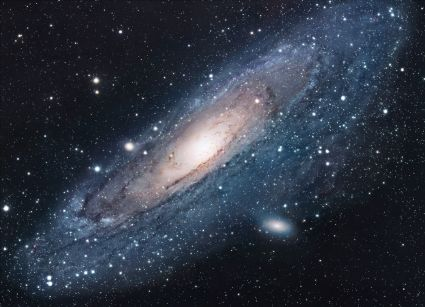
\includegraphics[width=0.5\textwidth]{figures/universe.jpg}
    \caption{This is an example image}
    \label{fig:universe}
\end{figure}

Do \textbf{not} put any placement constraint on figures,
such as \texttt{[h]} or \texttt{[h!]}.
%
Same considerations apply for other floating elements 
(e.g. tables, algorithms, listings, etc.).

Do \textbf{not} use the \texttt{\textbackslash\textbackslash} or \texttt{\textbackslash newline} commands to break lines.

Just leave an empty line between two paragraphs to start a new one.
%
The new line will be automatically indented.
%
This is intended: it is the \LaTeX{} way to separate capoverses.

\section{Concept}\label{concept}

\subsection{Type of product}

GridSim is a distributed desktop application for energy micro-grid simulation, composed of
a backend simulation engine and a graphical client, which can be deployed either as a
single co-located process or as two independent, network-connected components.

More precisely, the product is a hybrid of two of the categories listed above:
\begin{itemize}
    \item A \textbf{desktop application} with a graphical user interface (GUI), built with ScalaFX,
  through which the user creates micro-grid scenarios, starts/pauses/steps the simulation,
  and visualizes its evolution as an interactive, real-time graph (nodes = energy entities,
  edges = cables), together with dashboards and per-element detail panels (battery state of
  charge, solar panel irradiance, instantaneous power flow on a cable, etc.).
  \item A \textbf{backend service}, built on top of an actor system (Apache Pekko), that
  hosts the actual simulation engine, exposes an HTTP REST API to create/control simulations
  remotely, and publishes simulation telemetry on Apache Kafka topics so that one or more GUI
  clients can subscribe to the live state of a simulation without being co-located with the
  engine that computes it.
\end{itemize}

The two parts can run together in a single JVM process (local mode) or be split across different machines/processes
(distributed mode): a headless backend node (or cluster of nodes) running the simulation,
and one or more GUI clients connecting remotely via HTTP (control plane) and Kafka (data
plane). A Launcher component selects at startup which configuration to run (embedded,
backend-only, or remote GUI).

In addition to the interactive product, the project also provides a small embedded Domain
Specific Language (DSL), written in Scala, used to declaratively describe a micro-grid
scenario (houses, solar panels, batteries, cables, external grid, weather profile).

\subsection{Use case}

GridSim models a local energy micro-grid as a directed graph: nodes are energy entities
(houses, standalone solar panels, battery storages, and a single "External Grid" node
acting as an infinite source/sink), and edges are cables with a maximum power-transport
capacity. The simulation advances in discrete time steps ("ticks"); at every tick the
environment is updated, each entity resolves
its local energy balance (e.g., a house nets its consumption against its own solar
production and battery), and the residual surplus/deficit is routed through the micro-grid
topology using a power-flow algorithm, ultimately settling any
unbalanced energy with the External Grid. All intermediate states are kept immutable, so
the full history of a simulation run can be reconstructed and analyzed.

Users are not necessarily co-located with the machine running the simulation. The
simulation engine can run on a dedicated backend (e.g., a lab/cluster machine or a cloud VM
with more memory/CPU than a laptop), while the user interacts with it from a separate
desktop GUI, potentially from a different machine on the same network. This is a deliberate decoupling: the entity that computes the micro-grid is independent from the entity that observes/controls it.

Interaction happens in two distinct patterns always through the desktop GUI:
\begin{itemize}
    \item \textbf{Configuration phase} (low frequency, interactive): the user defines a scenario through the
    DSL/GUI — topology, components, weather, tick duration — before the simulation starts.
    This happens once per scenario, or occasionally during authoring/debugging of a scenario.
    \item \textbf{Monitoring/control phase} (continuous, real-time): once running, the system streams a new
    state snapshot at every tick; a user watching the GUI dashboard receives updates at the
    configured tick rate (potentially several times per second), observing the evolving graph,
    energy flows, and statistics, and can at any time issue start/pause/step commands. This is
    a long-lived, continuous interaction, not a one-shot request/response.
\end{itemize}

In this project, data is closer to "simulation state" than classic personal user data:
\begin{itemize}
    \item  \textbf{Scenario configuration} — authored/held client-side until a simulation is created on the backend.
    \item \textbf{Simulation state}, modeled as two parts: an immutable static model (topology, entity
    specifications) and dynamic state (environment, battery charge, flows), held by the backend actors.
    \item \textbf{Event history}: every state transition is persisted as an event (event sourcing) in a
    persistence journal, plus periodic snapshots, enabling crash recovery and historical
    reconstruction of a run.
    \item \textbf{Telemetry stream}: per-tick snapshots are also published to Kafka topics so that GUI
    clients (and, potentially, external analytics consumers) can observe simulation evolution
    without querying the backend state directly.
\end{itemize}

\subsection{Distribution motivations}

Distribution in GridSim is motivated by a combination of factors; the dominant ones are
resource sharing/separation of concerns and fault tolerance, with computation parallelism
and geographic distribution as secondary but still relevant drivers.

\begin{itemize}
    \item \textbf{Resource sharing and separation of concerns}. The simulation engine and the GUI have very
    different resource profiles and lifecycles: the engine is CPU/state-heavy and must run
    continuously and deterministically tick after tick, while the GUI is interaction-heavy and
    must stay responsive regardless of how expensive a tick computation is. By decoupling them
    (HTTP for control, Kafka for streaming telemetry), several GUI instances can observe the
    same backend simulation concurrently, a single backend can host multiple concurrent
    simulations, and a user is never forced to run the heavy simulation process on their own desktop, it can be hosted on a shared, more capable machine.
    \item \textbf{Computation speedup / parallelism}. A micro-grid is naturally decomposable: each entity
    (house, panel, storage) evolves largely independently within a tick, subject to the
    topology constraints resolved afterwards by the power-flow solver. This maps directly onto
    Pekko's cluster sharding: entities are distributed across (potentially many) shard regions
    and evolved concurrently, rather than sequentially in a single-threaded loop. This allows
    larger micro-grids (more entities) to be simulated and allows horizontal scaling by adding more
    backend nodes to the cluster as the simulated grid grows.
    \item \textbf{Fault tolerance}. Because the simulation state is valuable and the system is meant to run continuously, the architecture uses event sourcing (every state transition persisted as an event) plus periodic snapshotting, together with actor supervision strategies and automatic recovery on restart. This means an Entity or Simulation crash does not lose simulation history and the system can resume from the
    last known consistent state rather than failing the whole simulation.
    \item  \textbf{Geographic/organizational distribution}. the HTTP+Kafka boundary between GUI and backend is designed precisely so that a GUI client can be run anywhere with network access to the backend's exposed endpoints, which is relevant for scenarios such as a shared simulation server observed by multiple
    analysts from different workstations.
\end{itemize}

\section{Requirements Elicitation and Analysis}\label{requirements}

\begin{itemize}
  \item The requirements must explain \textbf{what} (not how) the software
  being produced should do.
  %
  \begin{itemize}
    \item you should not focus on the particular problems, but exclusively on
    what you want the application to do.
  \end{itemize}

  \item Requirements must be clearly identified, and possibly numbered

  \item Requirements are divided into:
  %
  \begin{itemize}
    \item \textbf{Functional}: some functionality the software should provide to the user

    \item \textbf{Non-functional}: requirements that do not directly concern behavioural aspects, such as consistency, availability, etc.

    \item \textbf{Implementation}: constrain the entire phase of system realization, 
    for instance by requiring the use of a specific programming language and/or a specific software tool
    %
    \begin{itemize}
      \item these constraints should be adequately justified by political / economic / administrative reasons\ldots{}
      \item \ldots{} otherwise, implementation choices should emerge \emph{as  a consequence of} design
    \end{itemize}
  \end{itemize}

  \item If there are domain-specific terms, these should be explained in a glossary
  
  \item Each requirement must have its own \textbf{acceptance criterion}
  %
  \begin{itemize}
    \item these will be important for the validation phase
  \end{itemize}
\end{itemize}

\subsection{Relevant Distributed System Features}
\label{ds-features}

Motivate which distributed system features are relevant for your project, and which are not.
%
\begin{itemize}
  \item transparency
  \begin{itemize}
    \item does your system need to hide distribution details from users or developers?
    \item is it important that failures, location, or replication are invisible?
  \end{itemize}

  \item fault tolerance, dependability -- availability, reliability, integrity, maintainability, safety
  \begin{itemize}
    \item what happens if a component fails? is uninterrupted service required?
    \item is data loss or corruption unacceptable?
    \item how quickly must the system recover from faults?
  \end{itemize}

  \item scalability
  \begin{itemize}
    \item will the system need to handle increasing numbers of users, requests, or data?
    \item is it expected to grow over time?
  \end{itemize}

  \item security, trust
  \begin{itemize}
    \item is sensitive data being processed or stored?
    \item are there multiple user roles with different permissions?
    \item is authentication or authorization required?
  \end{itemize}

  \item resource sharing
  \begin{itemize}
    \item do multiple users or components need access to shared resources?
    \item is coordination or synchronization needed?
  \end{itemize}

  \item openness, interoperability, heterogeneity of components
  \begin{itemize}
    \item Will your system interact with external systems or use components built with different technologies?
    \item Is standardization or compatibility important?
  \end{itemize}

  \item evolvability, maintainability
  \begin{itemize}
    \item Will the system need to be updated or extended after deployment?
    \item Is long-term maintenance a concern?
  \end{itemize}

  \item performance, concurrency, computation / communication efficiency, bandwidth
  \begin{itemize}
    \item Are there strict requirements on response time or throughput?
    \item Will many operations happen in parallel?
    \item Is network usage a concern?
  \end{itemize}

  \item economy, costs  
  \begin{itemize}
    \item Are there budget constraints for development, deployment, or operation?
    \item Is minimizing resource usage important?
  \end{itemize}
\end{itemize}

\section{Design}\label{design}

This chapter explains the strategies used to meet the requirements identified in the analysis. 
%
Ideally, the design should be the same, regardless of the technological choices made during the implementation phase.

\begin{quote}
You can re-arrange the sections as you prefer, but all the sections must be present in the end
\end{quote}

\noindent
\textbf{Important:} try to motivate your design choices in relation to the requirements and features identified 
in \cref{requirements} and \cref{ds-features}.

\subsection{Architecture}\label{architecture}

\begin{itemize}
  \item Which architectural style?
  %
  \begin{itemize}
    \item why?
  \end{itemize}
\end{itemize}

\subsection{Infrastructure}\label{infrastructure}

\begin{itemize}
  \item are there \emph{infrastructural components} that need to be introduced? \emph{how many}?
  %
  \begin{itemize}
    \item e.g.~\emph{clients}, \emph{servers}, \emph{load balancers},
    \emph{caches}, \emph{databases}, \emph{message brokers},
    \emph{queues}, \emph{workers}, \emph{proxies}, \emph{firewalls},
    \emph{CDNs}, \emph{etc.}
  \end{itemize}

  \item how do components \emph{distribute} over the network? \emph{where}?
  %
  \begin{itemize}
    \item e.g.~do servers / brokers / databases / etc. sit on the same
    machine? on the same network? on the same datacenter? on the same
    continent?
  \end{itemize}

  \item how do components \emph{find} each other?
  %
  \begin{itemize}
    \item how to \emph{name} components?
    \item e.g.~DNS, \emph{service discovery}, \emph{load balancing},
    \emph{etc.}
  \end{itemize}
\end{itemize}

\begin{quote}
Component diagrams are welcome here
\end{quote}

\subsection{Modelling}\label{modelling}

\begin{itemize}
  \item which \textbf{domain entities} are there?
  %
  \begin{itemize}
    \item e.g.~\emph{users}, \emph{products}, \emph{orders}, \emph{etc.}
  \end{itemize}
  
  \item how do \emph{domain entities} \textbf{map to} \emph{infrastructural components}?
  %
  \begin{itemize}
    \item e.g.~state of a video game on central server, while inputs/representations on clients
    \item e.g.~where to store messages in an IM app? for how long?
  \end{itemize}

  \item which \textbf{domain events} are there?
  %
  \begin{itemize}
    \item e.g.~\emph{user registered}, \emph{product added to cart}, \emph{order placed}, \emph{etc.}
  \end{itemize}
  
  \item which sorts of \textbf{messages} are exchanged?
  %
  \begin{itemize}
    \item e.g.~\emph{commands}, \emph{events}, \emph{queries}, \emph{etc.}
  \end{itemize}

  \item what information does the \textbf{state} of the system comprehend
  %
  \begin{itemize}
    \item e.g.~\emph{users' data}, \emph{products' data}, \emph{orders' data}, \emph{etc.}
  \end{itemize}
\end{itemize}

\begin{quote}
Class diagram are welcome here
\end{quote}

\subsection{Interaction}\label{interaction}

\begin{itemize}
  \item how do components \emph{communicate}? \emph{when}? \emph{what}?
  \item \emph{which} \textbf{interaction patterns} do they enact?
\end{itemize}

\begin{quote}
Sequence diagrams are welcome here
\end{quote}

\subsection{Behaviour}\label{behaviour}

\begin{itemize}
  \item how does \emph{each} component \textbf{behave} individually (e.g.~in \emph{response} to \emph{events} or messages)?
  \begin{itemize}
    \item some components may be \emph{stateful}, others \emph{stateless}
  \end{itemize}

  \item which components are in charge of updating the \textbf{state} of the system? \emph{when}? \emph{how}?
\end{itemize}

\begin{quote}
State diagrams are welcome here
\end{quote}

\subsection{Data and Consistency Issues}\label{data-and-consistency-issues}

\begin{itemize}
  \item Is there any data that needs to be stored?
  %
  \begin{itemize}
    \item \emph{what} data? \emph{where}? \emph{why}?
  \end{itemize}
  
  \item how should \emph{persistent data} be \textbf{stored}?
  %
  \begin{itemize}
    \item e.g.~relations, documents, key-value, graph, etc.
    \item why?
  \end{itemize}
  
  \item Which components perform queries on the database?
  %
  \begin{itemize}
    \item \emph{when}? \emph{which} queries? \emph{why}?
    \item concurrent read? concurrent write? why?
  \end{itemize}
  
  \item Is there any data that needs to be shared between components?
  %
  \begin{itemize}
    \item \emph{why}? \emph{what} data?
  \end{itemize}
\end{itemize}

\subsection{Fault-Tolerance}\label{fault-tolerance}

\begin{itemize}
  \item Is there any form of data \textbf{replication} / federation / sharing?
  %
  \begin{itemize}
    \item \emph{why}? \emph{how} does it work?
  \end{itemize}
  
  \item Is there any \textbf{heart-beating}, \textbf{timeout}, \textbf{retry mechanism}?
  %
  \begin{itemize}
    \item \emph{why}? \emph{among} which components? \emph{how} does it work?
  \end{itemize}
  
  \item Is there any form of \textbf{error handling}?
  %
  \begin{itemize}
    \item \emph{what} happens when a component fails? \emph{why}? \emph{how}?
  \end{itemize}
\end{itemize}

\subsection{Availability}\label{availability}

\begin{itemize}
  \item Is there any \textbf{caching} mechanism?
  %
  \begin{itemize}
    \item \emph{where}? \emph{why}?
  \end{itemize}
  
  \item Is there any form of \textbf{load balancing}?
  %
  \begin{itemize}
    \item \emph{where}? \emph{why}?
  \end{itemize}

  \item In case of \textbf{network partitioning}, how does the system behave?
  %
  \begin{itemize}
    \item \emph{why}? \emph{how}?
  \end{itemize}
\end{itemize}

\subsection{Security}\label{security}

\begin{itemize}
  \item Is there any form of \textbf{authentication}?
  %
  \begin{itemize}
    \item \emph{where}? \emph{why}?
  \end{itemize}

  \item Is there any form of \textbf{authorization}?
  %
  \begin{itemize}
    \item which sort of \emph{access control}?
    \item which sorts of users / \emph{roles}? which \emph{access rights}?
  \end{itemize}

  \item Are \textbf{cryptographic schemas} being used?
  %
  \begin{itemize}
    \item e.g.~token verification,
    \item e.g.~data encryption, etc.
  \end{itemize}
\end{itemize}

\section{Implementation}\label{implementation}

Please report here all the implementation (technology-dependent) choices you made while implementing your design.

\begin{quote}
  If you run out of time for this project, you may consider leaving some aspect unimplemented, 
  and simply discuss how you would have implemented them.
  %
  In this case, better would be to discuss unimplemented features in \cref{future-works}.
\end{quote}

\begin{itemize}
  \item which \textbf{network protocols} to use?
  %
  \begin{itemize}
    \item e.g.~UDP, TCP, HTTP, WebSockets, gRPC, XMPP, AMQP, MQTT, etc.
  \end{itemize}
  
  \item how should \emph{in-transit data} be \textbf{represented}?
  %
  \begin{itemize}
    \item e.g.~JSON, XML, YAML, Protocol Buffers, etc.
  \end{itemize}
  
  \item how should \emph{databases} be \textbf{queried}?
  %
  \begin{itemize}
    \item e.g.~SQL, NoSQL, etc.
  \end{itemize}
  
  \item how should components be \emph{authenticated}?
  %
  \begin{itemize}
    \item e.g.~OAuth, JWT, etc.
  \end{itemize}

  \item how should components be \emph{authorized}?
  %
  \begin{itemize}
    \item e.g.~RBAC, ABAC, etc.
  \end{itemize}
\end{itemize}

\subsection{Technological details}\label{technological-details}

\begin{itemize}
  \item any particular \emph{framework} / \emph{technology} being exploited goes here
\end{itemize}

\section{Validation}\label{validation}

\subsection{Automatic Testing}\label{automatic-testing}

\begin{itemize}
  \item how were individual components \textbf{\emph{unit}-test}ed?
  
  \item how was communication, interaction, and/or integration among components tested?
  
  \item how to \textbf{\emph{end-to-end}-test} the system?
  %
  \begin{itemize}
    \item e.g.~production vs.~test environment
  \end{itemize}

  \item for each test specify:
  %
  \begin{itemize}
    \item rationale of individual tests
    \item how were the test automated
    \item how to run them
    \item which requirement they are testing, if any
  \end{itemize}
\end{itemize}

\begin{quote}
recall that \emph{deployment} \textbf{automation} is commonly used to \emph{test} the system in \emph{production-like} environment
\end{quote}

\begin{quote}
recall to test corner cases (crashes, errors, etc.)
\end{quote}

\subsection{Acceptance test}\label{acceptance-test}

\begin{itemize}
  \item did you perform any \emph{manual} testing?
  %
  \begin{itemize}
    \item what did you test?
    \item why wasn't it automatic?
  \end{itemize}
\end{itemize}

\section{Deployment}\label{deployment}

\begin{itemize}
  \item should one install your software from scratch, how to do it?
  %
  \begin{itemize}
    \item provide instructions
    \item provide expected outcomes
  \end{itemize}

  \item what software should be installed on the machines to run your project? which versions?
  
  \item should one set environment variables or configuration files?
  
  \item if you're using containerization (e.g.~Docker), 
  describe how you engineered your deployment scrips (e.g. \texttt{docker-compose.yml} files)
\end{itemize}

\section{User Guide}\label{user-guide}

\begin{itemize}
  \item how to use your software?
  %
  \begin{itemize}
    \item provide instructions
    \item provide expected outcomes
    \item provide screenshots if possible
  \end{itemize}
\end{itemize}

\section{Self-evaluation}\label{self-evaluation}

\begin{itemize}
  \item An individual section is required for each member of the group
  \item Each member must self-evaluate their work, listing the strengths and weaknesses of the product
  \item Each member must describe their role within the group as objectively as possible.
\end{itemize}

It should be noted that each student is only responsible for their own section.

\section{Future works}\label{future-works}

Discuss possible future works, improvements, extensions, optimizations, etc.

Also discuss here any unimplemented feature, and how you would have implemented it.

\bibliographystyle{plain}
\bibliography{references}

\end{document}
